%% -*- mode: LaTeX; TeX-master: "../EndOfYear11.tex" -*-
\newcommand{\fixme}{\color{red} FIXME!}

\tausection{Combination of upper limits on tau LFV branching fractions}
\cutname{lfv-limits-combinations.html}
\label{sec:tau:lfv_com}
\def\cls{$CL_s$}

In this section we report on our combination of upper limits of tau LFV branching fractions. We would like stress out that most of the searches listed in~\ref{tab:tau:lfv-upper-limits} observed a downward fluctuation. Since downward fluctuations in Feldmann-Cousinus~\cite{PhysRevD.57.3873} can lead to artificial low exclusions~\cite{PhysRevD.86.010001} on branching fractions we choose to \cls \cite{Mistlberger:2012rs} method which alleviates this effect. \\
\cls method is based on two hypothesis: signal + background and background only. We calculate observed confidence levels for the two hypothesis:
\begin{align}
CL_{s+b} = P_{s+b}(Q \leq Q_{obs}) = \int_{- \infty}^{Q_{obs}} \frac{dP_{s+b}}{dQ} dQ,\\
CL_{b} = P_{b}(Q \leq Q_{obs}) = \int_{- \infty}^{Q_{obs}} \frac{dP_{b}}{dQ} dQ,
\label{pdfs}
\end{align}
where $CL_{s+b}$ is confidence level observed for signal + background hypothesis, $CL_{b}$ is confidence level observed for background only hypothesis, $\frac{dP_{s+b}}{dQ}$ and $\frac{dP_{b}}{dQ}$ are probability distribution functions (p.d.f.'s) for the two corresponding hypothesis and $Q$ is so called test statistics. \cls value is defined as normalized confidence level observed for signal plus background hypothesis to confidence level observed for background hypothesis:
\begin{equation}
CL_s=\dfrac{CL_{s+b}}{CL_{b}}.
\end{equation}\\
For multichannel searches the p.d.f.'s from~\ref{pdfs} become a product of individual p.d.f.'s for given experiment. One can write the \cls value explicit:
\begin{equation}
CL_s = \dfrac{\prod_{i=1}^{N_{chan}}\sum_{n=0}^{n_i} \dfrac{e^{-(s_i+b_i)} (s_i+b_i)^{n}}{n!} }{\prod_{i=1}^{n_{chan}}  \sum_{n=0}^{n_i} \dfrac{e^{-b_i} b_i^{n}}{n!}}    \dfrac{\prod_{j=1}^{n} s_iS_i(x_{ij})+b_iB_i(x_{ij})}{\prod_{j=1}^{n_i}B_i(x_{ij})},
\end{equation}
where $N_{chan}$ are number of channels, $n_i$ is the number of observed candidates in the $i^{th}$ channel, $x_{ij}$ are the values of discriminating variables, $s_i$ and $b_i$ are the number of signal and background events in the $i^{th}$ channel and $S_i$, $B_i$ are the probability distribution functions of the discriminating variables. \\
For the technical implementation we used an implementation provided by Tom Junk\cite{tjunk}. For each experiment we estimated the number of expected signal events using the formula:
\begin{equation}
\begin{split}
s_i & =2\mathcal{L}_i\sigma_{\tau\tau}Br(\tau \rightarrow LFV) \\
& =\frac{Br(\tau \rightarrow LFV)}{\alpha},
\end{split}
\end{equation}
where $\mathcal{L}_i$ is the integrated luminosity of an given experiment, $\sigma_{\tau\tau}$ is the cross section of a process $e^+ e^- \rightarrow  \tau^+ \tau^-$, $Br(\tau \rightarrow LFV)$ is the branching fraction of searched process and $\alpha$ is so called normalization factor\footnote{In case of LHCb results we take the the normalization directly from the appropriate paper.}. The systematics uncertainties are evaluated in pseudoexperiments generation by varying nuisance parameters($s_i$, $b_i$). The values are varied accordingly to Gaussian distribution width equal to corresponding systematic.\\
As mentioned at the begging most of the limits calculated by the B factories used Feldman-Cousin method, for comparison purposes in table~\ref{tab:tau:lfv-upper-limits_comb} we reported individual limits calculated with \cls method as well our combined limit. The same numbers are shown in Figure~\ref{fig:tau:lfv-limits-plot_average}. CLEO results were not taken into account because of negligible impact, also if a result between Belle an \babar is an order of magnitude stronger we did not perform a combination of this limits.



\begin{center}
\begin{longtable}{lcl@{}rl}

\caption{HFAG 2014  upper limit for the lepton flavor violating $\tau$ decay modes combinations. Individual experiments limits are recalculated using \cls method and final combination is reported. For convenience, the decay modes
are grouped in categories labelled according to their particle content. The label ``(L)'' in the category column means that the decay mode implies lepton number violation as well as the lepton flavor violation. ``BNV'' indicates that the channel is Baryon Number Violating.
\label{tab:tau:lfv-upper-limits_comb}}%
\\
\hline
\multicolumn{1}{l}{\bfseries Decay mode} &
\multicolumn{1}{l}{\bfseries Category} &
\multicolumn{2}{c}{\bfseries \begin{tabular}{@{}c@{}}90\% CL\\Limit\end{tabular}} &
\multicolumn{1}{l}{\bfseries Exp.}\\% &
%\multicolumn{1}{l}{\bfseries Ref.} \\
\hline
\endfirsthead
\multicolumn{5}{c}{{\bfseries \tablename\ \thetable{} -- continued from previous page}} \\ \hline
\multicolumn{1}{l}{\bfseries Decay mode} &
\multicolumn{1}{l}{\bfseries Category} &
\multicolumn{2}{c}{\bfseries \begin{tabular}{@{}c@{}}90\% CL\\Limit\end{tabular}} &
\multicolumn{1}{l}{\bfseries Exp.}\\% &
%\multicolumn{1}{l}{\bfseries Ref.} \\
\hline
\endhead
%
%  l\gamma
%   

\begin{ensuredisplaymath}
\Gamma_{156} =  {e^- \gamma} 
\end{ensuredisplaymath}
 &\(l\gamma\) & \( <\; \) &  \(5.4 \cdot 10^{-8}\)         & HFAG \\
 &            & \( <\; \) & \(22.0 \cdot 10^{-8}\)         & Belle \\
 &            & \( <\; \) & \(6.1 \cdot 10^{-8}\)         & \babar  \\ 
%\hline
\begin{ensuredisplaymath}
\Gamma_{157} =  {\mu^- \gamma} 
\end{ensuredisplaymath}
 &            & \( <\; \) &  \(5.0 \cdot 10^{-8}\)         & HFAG \\
 &            & \( <\; \) & \(17.0 \cdot 10^{-8}\)         & Belle  \\
 &            & \( <\; \) & \(5.9 \cdot 10^{-8}\)         & \babar   \\ 
\hline
%
%  lP0
\begin{ensuredisplaymath}
\Gamma_{160} =  {e^- K^0_S} 
\end{ensuredisplaymath}
 & \(lP^0 \)  & \( <\; \) & \(1.4 \cdot 10^{-8}\)         & HFAG  \\
 &            & \( <\; \) & \(1.8 \cdot 10^{-8}\)         & Belle  \\
 &            & \( <\; \) & \(4.7 \cdot 10^{-8}\)         & \babar   \\ 
%\hline
\begin{ensuredisplaymath}
\Gamma_{161} =  {\mu^- K^0_S} 
\end{ensuredisplaymath}
 &            & \( <\; \) & \(1.5 \cdot 10^{-8}\)         & HFAG  \\
&            & \( <\; \) & \(1.7 \cdot 10^{-8}\)         & Belle  \\
 &            & \( <\; \) & \(6.9 \cdot 10^{-8}\)         & \babar   \\ 
\hline
%
% l V0
%
\begin{ensuredisplaymath}
\Gamma_{164} =  {e^- \rho^0} 
\end{ensuredisplaymath}
 &  \(l V^0\) & \( <\; \) & \(1.5 \cdot 10^{-8}\)         & HFAG  \\
 &            & \( <\; \) & \(1.9 \cdot 10^{-8}\)         & Belle\\
 &            & \( <\; \) & \(5.2 \cdot 10^{-8}\)         & \babar   \\ 
%\hline
\begin{ensuredisplaymath}
\Gamma_{165} =  {\mu^- \rho^0} 
\end{ensuredisplaymath}
 &            & \( <\; \) & \(1.5 \cdot 10^{-8}\)         & HFAG  \\
 &            & \( <\; \) & \(2.1 \cdot 10^{-8}\)         & Belle\\
 &            & \( <\; \) & \(6.2 \cdot 10^{-8}\)         & \babar \\ 
%\hline
\begin{ensuredisplaymath}
\Gamma_{168} =  {e^- K^*(892)^0} 
\end{ensuredisplaymath}
 &            & \( <\; \) & \(2.3 \cdot 10^{-8}\)         & HFAG \\
 &            & \( <\; \) & \(3.4 \cdot 10^{-8}\)         & Belle \\
 &            & \( <\; \) & \(6.1 \cdot 10^{-8}\)         & \babar   \\ 
%\hline
\begin{ensuredisplaymath}
\Gamma_{169} =  {\mu^- K^*(892)^0} 
\end{ensuredisplaymath}
 &            & \( <\; \) & \(6.0 \cdot 10^{-8}\)         & HFAG \\
 &            & \( <\; \) & \(6.6 \cdot 10^{-8}\)         & Belle \\
 &            & \( <\; \) & \(17.0 \cdot 10^{-8}\)         & \babar   \\ 
%\hline
\begin{ensuredisplaymath}
\Gamma_{170} =  {e^- \bar{K}^*(892)^0} 
\end{ensuredisplaymath}
 &            & \( <\; \) & \(2.2 \cdot 10^{-8}\)         & HFAG \\
 &            & \( <\; \) & \(3.3 \cdot 10^{-8}\)         & Belle \\
 &            & \( <\; \) & \(5.6 \cdot 10^{-8}\)         & \babar   \\ 
%\hline
\begin{ensuredisplaymath}
\Gamma_{171} =  {\mu^- \bar{K}^*(892)^0} 
\end{ensuredisplaymath}
 &            & \( <\; \) & \(4.2 \cdot 10^{-8}\)         & HFAG  \\
 &            & \( <\; \) & \(6.3 \cdot 10^{-8}\)         & Belle  \\
 &            & \( <\; \) & \(9.1 \cdot 10^{-8}\)         & \babar \\ 
%\hline

\begin{ensuredisplaymath}
\Gamma_{176} =  {e^- \phi} 
\end{ensuredisplaymath}
 &            & \( <\; \) & \(2.0 \cdot 10^{-8}\)         & HFAG \\
 &            & \( <\; \) & \(3.5 \cdot 10^{-8}\)         & Belle \\
 &            & \( <\; \) & \(4.3 \cdot 10^{-8}\)         & \babar   \\ 
%\hline
\begin{ensuredisplaymath}
\Gamma_{177} =  {\mu^- \phi} 
\end{ensuredisplaymath}
 &            & \( <\; \) &\(6.8 \cdot 10^{-8}\)         & HFAG \\
 &            & \( <\; \) &\(7.6 \cdot 10^{-8}\)         & Belle  \\
 &            & \( <\; \) & \(18.0 \cdot 10^{-8}\)         & \babar   \\ 
%\hline
\begin{ensuredisplaymath}
\Gamma_{166} =  {e^- \omega} 
\end{ensuredisplaymath}
 &            & \( <\; \) & \(3.3 \cdot 10^{-8}\)         & HFAG \\
 &            & \( <\; \) & \(5.2 \cdot 10^{-8}\)         & Belle  \\
 &            & \( <\; \) & \(9.4 \cdot 10^{-8}\)         & \babar    \\ 
%\hline
\begin{ensuredisplaymath}
\Gamma_{167} =  {\mu^- \omega} 
\end{ensuredisplaymath}
 &            & \( <\; \) & \(4.0 \cdot 10^{-8}\)         & HFAG \\
 &            & \( <\; \) & \(6.1 \cdot 10^{-8}\)         & Belle  \\
 &            & \( <\; \) &  \(10.0 \cdot 10^{-8}\)         & \babar   \\ 
\hline
%
% lll
%
\begin{ensuredisplaymath}
\Gamma_{178} =  {e^- e^+ e^-} 
\end{ensuredisplaymath}
 &  \(lll\)   & \( <\; \) & \(1.4 \cdot 10^{-8}\)         & HFAG \\
 &            & \( <\; \) & \(2.7 \cdot 10^{-8}\)         & Belle  \\
 &            & \( <\; \) & \(3.1 \cdot 10^{-8}\)         & \babar    \\ 
%\hline
\begin{ensuredisplaymath}
\Gamma_{181} =  {\mu^- e^+ e^-} 
\end{ensuredisplaymath}
 &            & \( <\; \) & \(1.1 \cdot 10^{-8}\)         & HFAG \\
 &            & \( <\; \) & \(1.7 \cdot 10^{-8}\)         & Belle \\
 &            & \( <\; \) & \(3.0 \cdot 10^{-8}\)         & \babar    \\ 
%\hline
\begin{ensuredisplaymath}
\Gamma_{179} =  {e^- \mu^+ \mu^-} 
\end{ensuredisplaymath}
 &            & \( <\; \) & \(1.6 \cdot 10^{-8}\)         & HFAG \\
 &            & \( <\; \) & \(2.6 \cdot 10^{-8}\)         & Belle  \\
 &            & \( <\; \) & \(4.1 \cdot 10^{-8}\)         & \babar     \\ 
%\hline
\begin{ensuredisplaymath}
\Gamma_{183} =  {\mu^- \mu^+ \mu^-} 
\end{ensuredisplaymath}
 &            & \( <\; \) & \(1.2 \cdot 10^{-8}\)         & HFAG \\
 &            & \( <\; \) & \(2.1 \cdot 10^{-8}\)         & Belle\\
 &            & \( <\; \) & \(4.0 \cdot 10^{-8}\)         & \babar  \\ 
 &            & \( <\; \) & \(4.6 \cdot 10^{-8}\)         & \lhcb   \\ 

%\hline
\begin{ensuredisplaymath}
\Gamma_{182} =  {e^- \mu^+ e^-} 
\end{ensuredisplaymath}
 &            & \( <\; \) & \(8.4 \cdot 10^{-9}\)         & HFAG \\
 &            & \( <\; \) & \(1.4 \cdot 10^{-8}\)         & Belle  \\
 &            & \( <\; \) & \(2.1 \cdot 10^{-8}\)         & \babar    \\ 
%\hline
\begin{ensuredisplaymath}
\Gamma_{180} =  {\mu^- e^+ \mu^-} 
\end{ensuredisplaymath}
 &            & \( <\; \) & \(9.8 \cdot 10^{-9}\)         & HFAG \\
 &            & \( <\; \) & \(1.6 \cdot 10^{-8}\)         & Belle \\
 &            & \( <\; \) & \(2.6 \cdot 10^{-8}\)         & \babar     \\ 
 %
% Lambda h
%
\hline
\begin{ensuredisplaymath}
\Gamma_{211} =  { \pi^- \Lambda } 
\end{ensuredisplaymath}
& BNV & \( <\; \) & \(1.9 \cdot 10^{-8}\)         & HFAG  \\
&                & \( <\; \) & \(3.2 \cdot 10^{-8}\)         & Belle  \\
 &               & \( <\; \) & \(6.7 \cdot 10^{-8}\)        & \babar     \\  
%\hline
\begin{ensuredisplaymath}
\Gamma_{212} =  { \pi^- \bar{\Lambda}} 
\end{ensuredisplaymath}
 &            & \( <\; \) & \(1.8 \cdot 10^{-9}\)         & HFAG \\
 &            & \( <\; \) & \(2.9 \cdot 10^{-8}\)         & Belle  \\
 &            & \( <\; \) & \(6.5 \cdot 10^{-8}\)        & \babar     \\  
%\hline
\begin{ensuredisplaymath}
\Gamma_{213} =  { K^- \Lambda } 
\end{ensuredisplaymath}
 &            & \( <\; \) & \(3.7 \cdot 10^{-9}\)         & HFAG \\
 &            & \( <\; \) & \(4.4 \cdot 10^{-8}\)         & Belle  \\
 &            & \( <\; \) & \(9.2\cdot 10^{-8}\)         & \babar     \\  
%\hline
\begin{ensuredisplaymath}
\Gamma_{214} =  { K^- \bar{\Lambda}} 
\end{ensuredisplaymath}
 &            & \( <\; \) & \(2.0 \cdot 10^{-9}\)         & HFAG \\
 &            & \( <\; \) & \(3.4 \cdot 10^{-8}\)         & Belle \\
 &            & \( <\; \) & \(5.0 \cdot 10^{-8}\)         & \babar     \\  
\hline 
\end{longtable}
\end{center}



\begin{figure}[tb]
  \begin{center}

    
    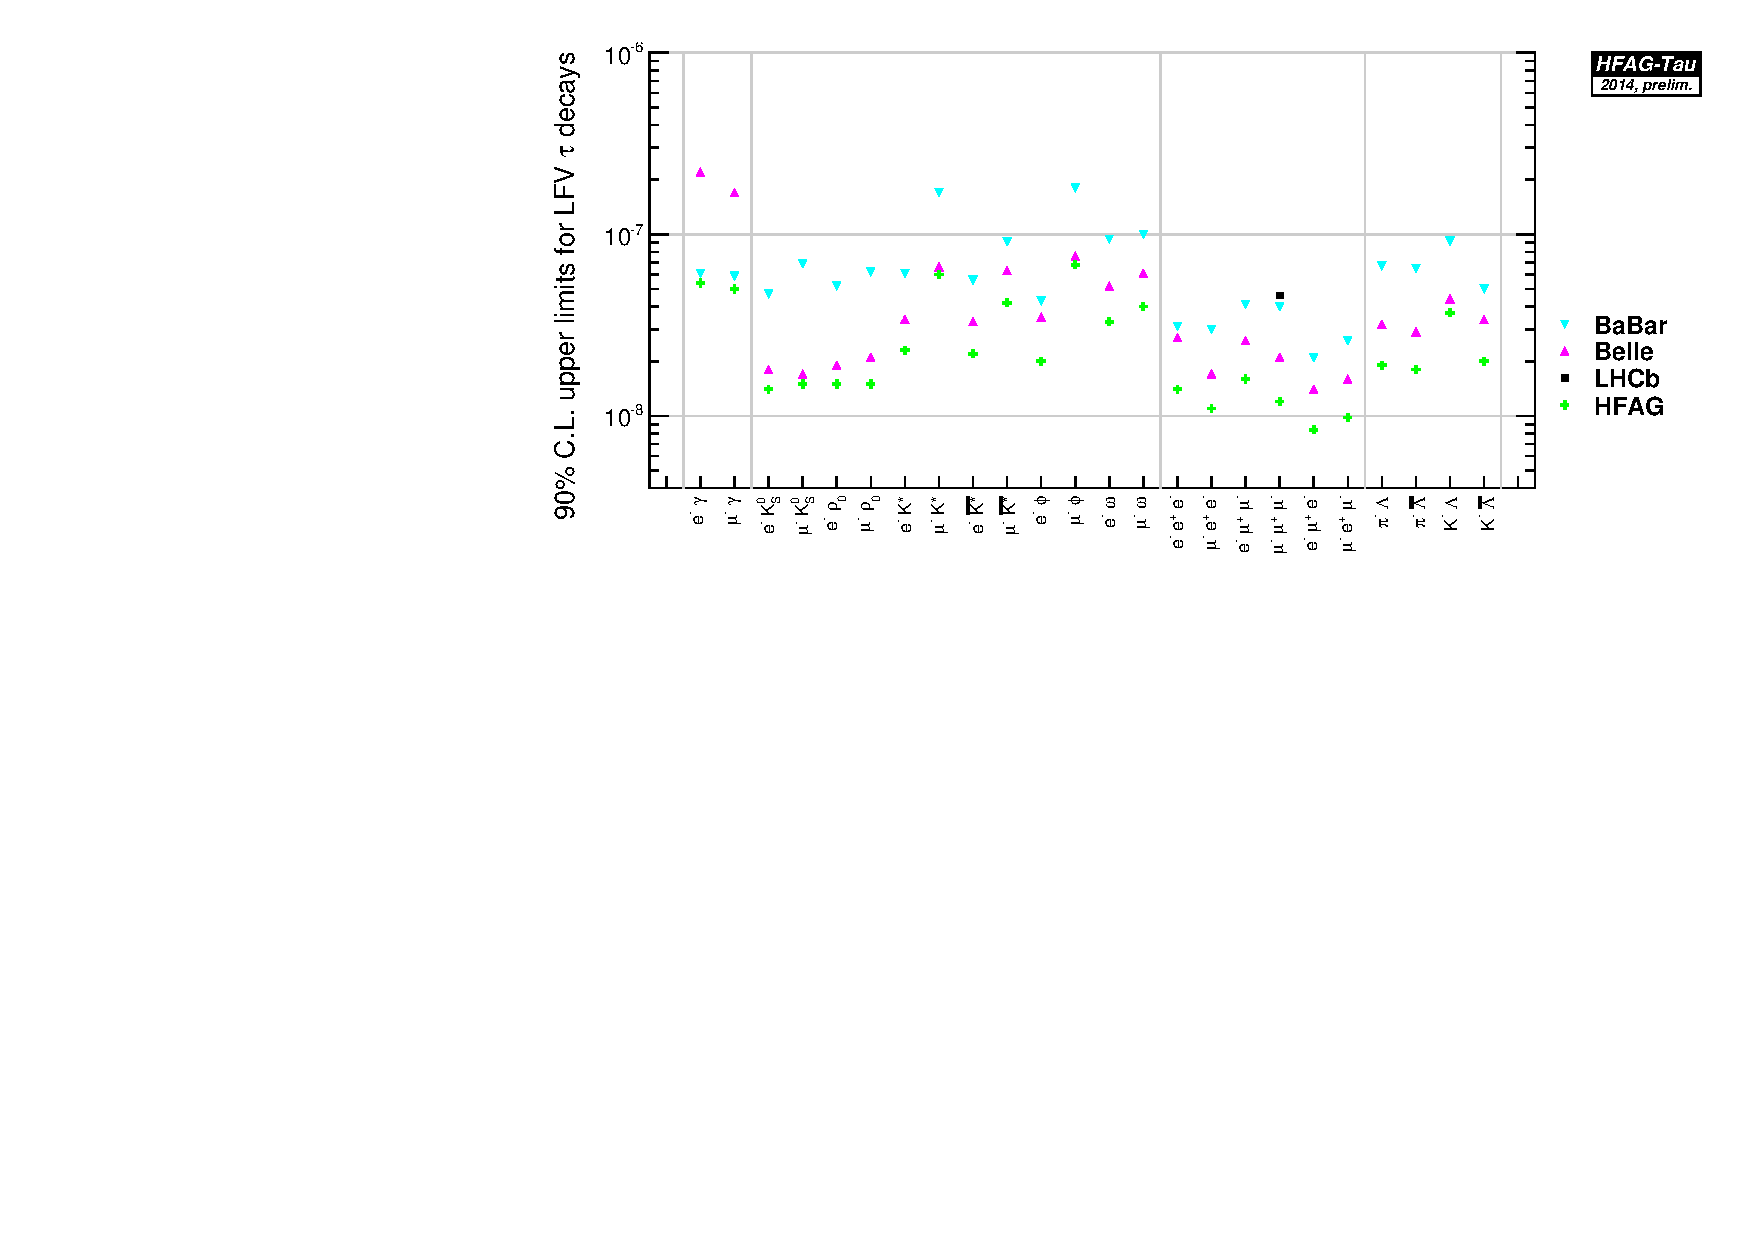
\includegraphics[angle=270,totalheight=0.9\textheight,clip]{figures/tau/TauLFV_UL_2013001_averaged.pdf}
    
    \caption{Tau lepton-flavour-violating branching fraction upper combination.
      \label{fig:tau:lfv-limits-plot_average}
    }
  \end{center}
\end{figure}
